\documentclass[12pt]{article}
\usepackage[margin=1.0in]{geometry}
\usepackage[utf8]{inputenc}
\usepackage[T1]{fontenc}
\usepackage{lmodern}
\usepackage[spanish]{babel}
\usepackage{amsmath}
\usepackage{graphicx}

\title{\LaTeX\ \textsc{notas}}

\begin{document}
\date{}
\maketitle


\LaTeX. es un programa diseñado con el proposito de crear documentos (libros, artículos, esritos etc.) en un ambiente matemático.
 
\begin{center}
\section*{Primeros pasos con \LaTeX}
\end{center}

Hay tres linéas fundamentales que todo texto en \LaTeX\ debe tener:\\

\begin{center}
\begin{verbatim}
\documentclass[12pt]{article}
\begin{document}

Aca va mi articulo

\end{document}
\end{verbatim}
\end{center}

La primera le dice al programa que clase de documento se va a escribir, en este caso es un art\'iculo.
La segunda indica el inicio del documento mientras que la tercera denota el fin del documento. Entre la segunda 
y la tercera linéa va a ir todo nuestro documento.

\begin{center}
\section*{Margenes:}
\end{center}

Para editar las margenes hay que usar el siguiente paquete:\\

\verb"\usepackage[margin=1.0in]{geometry}"
Donde \verb"margin" es el valor en pulgadas de la margen.


\section*{Idioma:}


Para cambiar de idioma se deben incluir los siguientes paquetes:\\
\verb"\usepackage[utf8]{inputenc}"\\
\verb"\usepackage[T1]{fontenc}"\\
\verb"\usepackage{lmodern}"\\
\verb"\usepackage[spanish]{babel}"\\

\begin{center}
\section*{Tipo de letra y tamaño}
\end{center}


\subsection*{Tipo de letra}


\LaTeX\ 	 trae predeterminadas 7 tipos de letras que son:\\
\verb"\textbf" \textbf{Hola}\\
\verb"\textit" \textit{Hola}\\
\verb"\textsc" \textsc{Hola}\\
\verb"\textsf" \textsf{Hola}\\
\verb"\textsl" \textsl{Hola}\\
\verb"\texttt" \texttt{Hola}\\
\verb"\textrm" \textrm{Hola}\\

\subsection*{Tamaño de letra}

Para cambiar el tamaño de la letra se debe usar la siguiente sintaxis:\\

\begin{verbatim}
\begin{size}
Hola
\end{size}
\end{verbatim}

Donde \verb"size" puede ser:\\

\begin{center}

\begin{tiny}
tiny
\end{tiny} 

\begin{scriptsize}
scriptsize
\end{scriptsize}

\begin{footnotesize}
footnotesize
\end{footnotesize}

\begin{small}
small
\end{small}

\begin{normalsize}
normalsize
\end{normalsize}

\begin{large}
large
\end{large}

\begin{Large}
Large
\end{Large}

\begin{LARGE}
LARGE
\end{LARGE}

\begin{huge}
huge
\end{huge}

\begin{Huge}
Huge
\end{Huge}

\end{center}

\begin{center}
\section*{Secciones}
\end{center}

Para crear secciones dentro de un documento usamos:

\begin{verbatim}
\section{Nombre de la secci\'on}
\end{verbatim}

Por ejemplo esta seccion se llama \textbf{Secciones}.

Tambien podemos crear subsecciones \& subsubsecciones:



\subsection{Soy una subsección}
\begin{verbatim}
\subsection{Nombre de la subsecci\'on}
\end{verbatim}

\subsubsection{Soy una subsubsección}
\begin{verbatim}
\subsubsection{Nombre de la subsubseccion}
\end{verbatim}

\begin{center}
\section*{Ecuaciones y simbolos matem\'aticos}
\end{center}

\subsection*{Simbolos matem\'aticos:}

En general los simbolos matem\'aticos empiezan con un \verb" \" , por ejemplo algunos de los simbolos
mas usados se escribiran:\\

\begin{center}
\begin{tabular}{|c|c|}
\hline
Simbolo & Sintaxis \\\hline
 $\pm$  & \verb"\pm" \\\hline
 $\mp$  & \verb"\mp" \\\hline
$\times$ & \verb"\times" \\\hline
$\div$ & \verb"\div" \\\hline
$\leq$ & \verb"\leq" \\\hline
$\geq$ & \verb"\geq" \\\hline
$\equiv$ & \verb"\equiv" \\\hline
$\simeq$ & \verb"\simeq" \\\hline
$\sum$ & \verb"\sum" \\\hline
$\bigotimes$ & \verb"\bigotimes" \\\hline
$\int$ & \verb"\int" \\\hline
$\oint$ & \verb"\oint" \\\hline
$\partial$ & \verb"\partial" \\\hline
$\hbar$ & \verb"\hslash" \\\hline
$\forall$ & \verb"\forall" \\\hline
$\infty$ & \verb"\infty" \\\hline

\end{tabular}
\end{center}

\subsection*{Ecuaciones:}

Para introducir una ecuaci\'on en el texto primero debemos incluir el siguiente paquete:\\

\verb"\usepackage{amsmath}"

Y luego inicializar la ecuacion así:

\begin{verbatim}
\begin{equation}\label{eq:1.1}
\vec{F} = m \ddot{\vecx}
Esto es una ecuación
\end{equation}
\end{verbatim}

La anterior sintaxis arrojaria el siguiente resultado:

\begin{equation}\label{eq:1.1}
\vec{F} = m \ddot{\vec{x}}
\end{equation}

Donde el label me permire referenciar la ecuaci\'on desde cualquier parte del texto así Eq.\ref{eq:1.1}  

\section*{Figuras}

Es necesario incluir el paquete \verb"graphicx" para tener las herramientas basicas para hacer graficas.:

\verb"\usepackage{graphicx}"\\

Ahora pongamos una grafica:

\begin{verbatim}
\begin{figure}\label{fig:PhDComics}
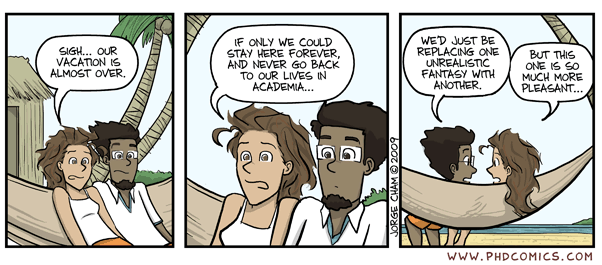
\includegraphics[scale=0.8]{f1.png}
\caption{Your vacations?}
\end{figure}
\end{verbatim}

\begin{figure}\label{fig:PhDComics}
\begin{center}
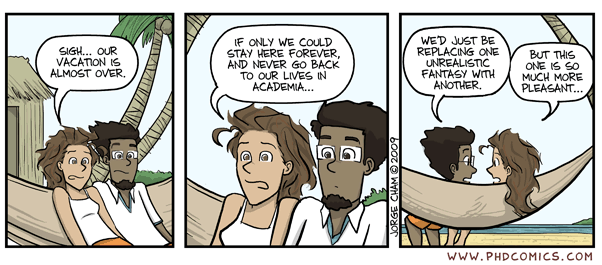
\includegraphics[scale=0.8]{f1.png}
\caption{Your vacations?}
\end{center}
\end{figure}

En la Fig.\ref{fig:PhDComics} vemos unas lindas vacaciones$!$

\section*{Tablas}

Ahora hagamos algunas tablas:

\begin{table}
\begin{center}
\begin{tabular}{|c|c|}
\hline
hola & que mas \\
\hline
\end{tabular}
\end{center}
\end{table}

\section*{Bibliograf\'ia}



%\begin{center}
\section*{Tips:}
%-\end{center}

\begin{itemize}
\item Para dejar un espacio distanciado entre lineas se debe usar \verb"\\" al final de cada linea.
\item Para escribir simbolos o ecuaciones matemáticas en el texto se debe usar el simbolo \$ \verb"$\dfrac{dx}{dt}$"   $\dfrac{dx}{dt}$
\item Para comentar lineas se utiliza el simbolo de porcentaje \%.



\begin{center}
\section*{Referencias:}
\end{center}

http://www.latex-tutorial.com/\\
http://www.latex-project.org/\\
http://www.latextemplates.com/
\end{itemize}

\end{document}

